\documentclass[11pt]{article}
\usepackage[T1]{fontenc}
\usepackage[utf8]{inputenc}
\usepackage[english]{babel}
\usepackage{amsmath,amssymb}
\usepackage{graphicx}
\usepackage{booktabs}
\usepackage{siunitx}
\usepackage[margin=1in]{geometry}
\usepackage[hidelinks]{hyperref}
\usepackage{caption}
\usepackage{xcolor}
\usepackage{tcolorbox}
\usepackage{natbib}
\captionsetup{font=small,labelfont=bf,justification=justified,singlelinecheck=false}
\sisetup{detect-weight=true,detect-family=true}
\newcommand{\pc}{\,\%}
\newcommand{\statusline}[2]{\texttt{#1}~\texttt{=}~\texttt{#2}}
\graphicspath{{../figures/}}

\newtcolorbox{statusbox}{colback=black!3,colframe=black!35,boxrule=0.4pt,
  left=6pt,right=6pt,top=5pt,bottom=5pt}

% GENERATED by code/emit_numbers.py from provenance/PAPER_NUMERICAL_RECONCILIATION.json.
% Do not edit. Every macro below is a value read from a hashed source file.

\newcommand{\rEightZeroStaticPredictedFrozen}{6.08276}% r80_static_predicted_frozen [_observables_exact.json]
\newcommand{\rEightZeroMobilePredictedFrozen}{8.544}% r80_mobile_predicted_frozen [_observables_exact.json]
\newcommand{\predictionStatus}{PRE\_\allowbreak{}RUN}% prediction_status [_observables_exact.json]
\newcommand{\freshStaticPredicted}{6.0076}% fresh_static_predicted [_adjudication.json]
\newcommand{\freshStaticObserved}{5.9991}% fresh_static_observed [_adjudication.json]
\newcommand{\freshStaticDeviationPercent}{-0.14}% fresh_static_deviation_percent [_adjudication.json]
\newcommand{\freshStaticCiNineFiveLow}{-1.05}% fresh_static_ci95_low [_adjudication.json]
\newcommand{\freshStaticCiNineFiveHigh}{0.77}% fresh_static_ci95_high [_adjudication.json]
\newcommand{\freshStaticPass}{\textsc{true}}% fresh_static_pass [_adjudication.json]
\newcommand{\freshMobilePredicted}{8.0574}% fresh_mobile_predicted [_adjudication.json]
\newcommand{\freshMobileObserved}{8.0771}% fresh_mobile_observed [_adjudication.json]
\newcommand{\freshMobileDeviationPercent}{0.24}% fresh_mobile_deviation_percent [_adjudication.json]
\newcommand{\freshMobileCiNineFiveLow}{-1.18}% fresh_mobile_ci95_low [_adjudication.json]
\newcommand{\freshMobileCiNineFiveHigh}{1.67}% fresh_mobile_ci95_high [_adjudication.json]
\newcommand{\freshMobilePass}{\textsc{true}}% fresh_mobile_pass [_adjudication.json]
\newcommand{\freshRatioPredicted}{1.3412}% fresh_ratio_predicted [_adjudication.json]
\newcommand{\freshRatioObserved}{1.3464}% fresh_ratio_observed [_adjudication.json]
\newcommand{\freshRatioDeviationPercent}{0.39}% fresh_ratio_deviation_percent [_adjudication.json]
\newcommand{\freshRatioCiNineFiveLow}{-1.30}% fresh_ratio_ci95_low [_adjudication.json]
\newcommand{\freshRatioCiNineFiveHigh}{2.07}% fresh_ratio_ci95_high [_adjudication.json]
\newcommand{\freshRatioPass}{\textsc{true}}% fresh_ratio_pass [_adjudication.json]
\newcommand{\equivalenceMarginPercent}{2.9}% equivalence_margin_percent [_adjudication.json]
\newcommand{\ratioOneExcluded}{\textsc{true}}% ratio_one_excluded [_adjudication.json]
\newcommand{\freshArmsRun}{28}% fresh_arms_run [_adjudication.json]
\newcommand{\freshArmsAnalysable}{28}% fresh_arms_analysable [_adjudication.json]
\newcommand{\freshArmsInvalid}{0}% fresh_arms_invalid [_adjudication.json]
\newcommand{\freshExtinctions}{0}% fresh_extinctions [_adjudication.json]
\newcommand{\blockedFractionXMean}{0.0004}% blocked_fraction_X_mean [_adjudication.json]
\newcommand{\radialProfileMaxAbsZ}{0.64}% radial_profile_max_abs_z [_residual.json]
\newcommand{\radialProfileRadiiTested}{15}% radial_profile_radii_tested [_residual.json]
\newcommand{\radialProfileMaxAbsDifference}{0.0038}% radial_profile_max_abs_difference [_residual.json]
\newcommand{\profileAgreesAtEveryRadius}{\textsc{true}}% profile_agrees_at_every_radius [_residual.json]
\newcommand{\historicalStaticMedianResidualPercent}{-1.83}% historical_static_median_residual_percent [_residual.json]
\newcommand{\historicalStaticMedianResidualN}{3}% historical_static_median_residual_n [_residual.json]
\newcommand{\historicalStaticMedianResidualZ}{-1.51}% historical_static_median_residual_z [_residual.json]
\newcommand{\historicalMobileMedianResidualPercent}{-5.10}% historical_mobile_median_residual_percent [_residual.json]
\newcommand{\historicalMobileMedianResidualN}{116}% historical_mobile_median_residual_n [_residual.json]
\newcommand{\historicalMobileMedianResidualZ}{-16.57}% historical_mobile_median_residual_z [_residual.json]
\newcommand{\historicalStaticMeanResidualPercent}{-1.39}% historical_static_mean_residual_percent [_residual.json]
\newcommand{\historicalStaticMeanResidualN}{3}% historical_static_mean_residual_n [_residual.json]
\newcommand{\historicalStaticMeanResidualZ}{-0.76}% historical_static_mean_residual_z [_residual.json]
\newcommand{\iidStaticPopulationREightZero}{6.08276}% iid_static_population_r80 [_residual.json]
\newcommand{\iidStaticMedianSummary}{6.00939}% iid_static_median_summary [_residual.json]
\newcommand{\iidStaticMedianRatio}{0.9879}% iid_static_median_ratio [_residual.json]
\newcommand{\iidStaticMeanRatio}{0.9859}% iid_static_mean_ratio [_residual.json]
\newcommand{\iidMobilePopulationREightZero}{8.544}% iid_mobile_population_r80 [_residual.json]
\newcommand{\iidMobileMedianSummary}{8.43236}% iid_mobile_median_summary [_residual.json]
\newcommand{\iidMobileMedianRatio}{0.9869}% iid_mobile_median_ratio [_residual.json]
\newcommand{\iidMobileMeanRatio}{0.9905}% iid_mobile_mean_ratio [_residual.json]
\newcommand{\dispersionStaticWithinArmSd}{0.737}% dispersion_static_within_arm_sd [_residual.json]
\newcommand{\dispersionMobileWithinArmSd}{1.780}% dispersion_mobile_within_arm_sd [_residual.json]
\newcommand{\dispersionStaticWithinArmSkew}{0.313}% dispersion_static_within_arm_skew [_residual.json]
\newcommand{\dispersionMobileWithinArmSkew}{1.072}% dispersion_mobile_within_arm_skew [_residual.json]
\newcommand{\dispersionIidStaticWithinArmSd}{0.668}% dispersion_iid_static_within_arm_sd [_residual.json]
\newcommand{\dispersionIidMobileWithinArmSd}{0.774}% dispersion_iid_mobile_within_arm_sd [_residual.json]
\newcommand{\ablationObservedMobileMedian}{8.0771}% ablation_observed_mobile_median [_adjudication.json]
\newcommand{\ablationPredFull}{8.0574}% ablation_pred_full [_adjudication.json]
\newcommand{\ablationPredNoShared}{8.3746}% ablation_pred_no_shared [_adjudication.json]
\newcommand{\ablationPredPoisson}{8.1660}% ablation_pred_poisson [_adjudication.json]
\newcommand{\ablationPredIdeal}{8.5440}% ablation_pred_ideal [_adjudication.json]
\newcommand{\ablationDistFull}{0.0197}% ablation_dist_full [_adjudication.json]
\newcommand{\ablationDistNoShared}{0.2975}% ablation_dist_no_shared [_adjudication.json]
\newcommand{\ablationDistPoisson}{0.0889}% ablation_dist_poisson [_adjudication.json]
\newcommand{\mSixVerdict}{{"M6\_\allowbreak{}REPRODUCES\_\allowbreak{}THE\_\allowbreak{}MOBILE\_\allowbreak{}MEDIAN\_\allowbreak{}RESIDUAL": true, "M6\_\allowbreak{}REPRODUCES\_\allowbreak{}THE\_\allowbreak{}STATIC\_\allowbreak{}MEDIAN\_\allowbreak{}RESIDUAL": true, "M6\_\allowbreak{}REPRODUCES\_\allowbreak{}THE\_\allowbreak{}MEAN\_\allowbreak{}SUMMARY\_\allowbreak{}AS\_\allowbreak{}NEARLY\_\allowbreak{}UNBIASED": true, "SHARED\_\allowbreak{}TRAJECTORY\_\allowbreak{}IS\_\allowbreak{}NECESSARY": true, "BIRTH\_\allowbreak{}FLUX\_\allowbreak{}ENDOGENEITY\_\allowbreak{}IS\_\allowbreak{}MATERIAL": true, "INTERACTION\_\allowbreak{}IS\_\allowbreak{}MATERIAL": false}}% m6_verdict [_m6.json]
\newcommand{\birthFluxVarianceOverMean}{1.285}% birth_flux_variance_over_mean [_mechanisms.json]
\newcommand{\capacityPerLifetimeOfferedHops}{25.5557}% capacity_per_lifetime_offered_hops [_mechanisms.json]
\newcommand{\capacityPerLifetimeExpectedRefusals}{0.00908288}% capacity_per_lifetime_expected_refusals [_mechanisms.json]
\newcommand{\budgetArmsPerCondition}{14}% budget_arms_per_condition [_freeze.json]
\newcommand{\budgetHardCapTotalArms}{28}% budget_hard_cap_total_arms [_freeze.json]
\newcommand{\budgetNoSeedReplacement}{\textsc{true}}% budget_no_seed_replacement [_freeze.json]
\newcommand{\pHop}{0.102633}% p_hop [_freeze.json]
\newcommand{\muX}{0.004}% mu_X [_freeze.json]
\newcommand{\ablationNoSharedTrajectoryMedianResidualPercent}{-1.983}% ablation_no_shared_trajectory_median_residual_percent [_m6.json]
\newcommand{\ablationNoSharedTrajectoryWithinArmSd}{0.7663}% ablation_no_shared_trajectory_within_arm_sd [_m6.json]
\newcommand{\ablationNoSharedTrajectoryLosesPercentagePoints}{-3.712}% ablation_no_shared_trajectory_loses_percentage_points [_m6.json]
\newcommand{\ablationPoissonBirthsMedianResidualPercent}{-4.424}% ablation_poisson_births_median_residual_percent [_m6.json]
\newcommand{\ablationPoissonBirthsWithinArmSd}{1.732}% ablation_poisson_births_within_arm_sd [_m6.json]
\newcommand{\ablationPoissonBirthsLosesPercentagePoints}{-1.271}% ablation_poisson_births_loses_percentage_points [_m6.json]
\newcommand{\cellStaticMedianObservedPercent}{-1.833}% cell_static_median_observed_percent [_m6.json]
\newcommand{\cellStaticMedianSurrogatePercent}{-1.206}% cell_static_median_surrogate_percent [_residual.json]
\newcommand{\cellStaticMedianConstructionPercent}{-1.235}% cell_static_median_construction_percent [_m6.json]
\newcommand{\cellStaticMeanObservedPercent}{-1.395}% cell_static_mean_observed_percent [_m6.json]
\newcommand{\cellStaticMeanSurrogatePercent}{-1.412}% cell_static_mean_surrogate_percent [_residual.json]
\newcommand{\cellStaticMeanConstructionPercent}{-1.485}% cell_static_mean_construction_percent [_m6.json]
\newcommand{\cellMobileMedianObservedPercent}{-5.172}% cell_mobile_median_observed_percent [_m6.json]
\newcommand{\cellMobileMedianSurrogatePercent}{-1.307}% cell_mobile_median_surrogate_percent [_residual.json]
\newcommand{\cellMobileMedianConstructionPercent}{-5.695}% cell_mobile_median_construction_percent [_m6.json]
\newcommand{\cellMobileMeanObservedPercent}{-0.5752}% cell_mobile_mean_observed_percent [_m6.json]
\newcommand{\cellMobileMeanSurrogatePercent}{-0.9512}% cell_mobile_mean_surrogate_percent [_residual.json]
\newcommand{\cellMobileMeanConstructionPercent}{-1.866}% cell_mobile_mean_construction_percent [_m6.json]
\newcommand{\radialProfileStaticMaxAbsZ}{8.904}% radial_profile_static_max_abs_z [_residual.json]
\newcommand{\radialProfileStaticMaxAbsDifference}{0.03407}% radial_profile_static_max_abs_difference [_residual.json]
\newcommand{\radialProfileStaticArms}{3}% radial_profile_static_arms [_residual.json]
\newcommand{\radialProfileMobileArms}{116}% radial_profile_mobile_arms [_residual.json]
\newcommand{\radialProfileFlagScope}{MOBILE\_\allowbreak{}ONLY}% radial_profile_flag_scope [_residual.json]
\newcommand{\secondaryMeanSummaryStaticPredicted}{-1.485}% secondary_mean_summary_static_predicted [_adjudication.json]
\newcommand{\secondaryMeanSummaryStaticObservedPercent}{-1.24}% secondary_mean_summary_static_observed_percent [_adjudication.json]
\newcommand{\secondaryMeanSummaryMobilePredicted}{-1.866}% secondary_mean_summary_mobile_predicted [_adjudication.json]
\newcommand{\secondaryMeanSummaryMobileObservedPercent}{-1.648}% secondary_mean_summary_mobile_observed_percent [_adjudication.json]
\newcommand{\secondaryWithinArmSdStaticPredicted}{0.6667}% secondary_within_arm_sd_static_predicted [_adjudication.json]
\newcommand{\secondaryWithinArmSdStaticObserved}{0.6985}% secondary_within_arm_sd_static_observed [_adjudication.json]
\newcommand{\secondaryWithinArmSdMobilePredicted}{1.681}% secondary_within_arm_sd_mobile_predicted [_adjudication.json]
\newcommand{\secondaryWithinArmSdMobileObserved}{1.645}% secondary_within_arm_sd_mobile_observed [_adjudication.json]
\newcommand{\secondaryWithinArmSkewMobileObserved}{0.8775}% secondary_within_arm_skew_mobile_observed [_adjudication.json]
\newcommand{\secondaryWithinArmSkewStaticObserved}{0.2473}% secondary_within_arm_skew_static_observed [_adjudication.json]
\newcommand{\marginModelErrorQuadraturePercent}{0.6352}% margin_model_error_quadrature_percent [_freeze.json]
\newcommand{\marginTwoSamplingSePercent}{2.219}% margin_two_sampling_se_percent [_freeze.json]
\newcommand{\marginMSixMonteCarloSeStaticPercent}{0.2754}% margin_M6_monte_carlo_se_static_percent [_freeze.json]
\newcommand{\marginMSixMonteCarloSeMobilePercent}{0.6024}% margin_M6_monte_carlo_se_mobile_percent [_freeze.json]
\newcommand{\marginCapacityCertifiedErrorOnREightZeroPercent}{0.01777}% margin_capacity_certified_error_on_r80_percent [_freeze.json]
\newcommand{\marginIntraStepOrderResidualPercent}{0.2008}% margin_intra_step_order_residual_percent [_freeze.json]
\newcommand{\marginHistoricalArmToArmRelativeSdStaticPercent}{2.11}% margin_historical_arm_to_arm_relative_sd_static_percent [_freeze.json]
\newcommand{\marginHistoricalArmToArmRelativeSdMobilePercent}{4.152}% margin_historical_arm_to_arm_relative_sd_mobile_percent [_freeze.json]
\newcommand{\marginSamplingSeAtOneFourArmsStaticPercent}{0.5639}% margin_sampling_se_at_14_arms_static_percent [_freeze.json]
\newcommand{\marginSamplingSeAtOneFourArmsMobilePercent}{1.11}% margin_sampling_se_at_14_arms_mobile_percent [_freeze.json]
\newcommand{\methodsCoreHash}{6676a35f\allowbreak{}b79d554d\allowbreak{}99da2b48\allowbreak{}e69b43f2\allowbreak{}d3c70f5a\allowbreak{}0f5cbacb\allowbreak{}2d258d56\allowbreak{}a83dd76c}% methods_core_hash [_freeze.json]
\newcommand{\methodsCoreHashStatus}{FROZEN}% methods_core_hash_status [_freeze.json]
\newcommand{\mSixSequentialStepZeroBaselineMTwoLevel}{-0.6563}% m6_sequential_step_0_baseline_M2_level [_m6.json]
\newcommand{\mSixSequentialStepOneAddSharedTrajectory}{-4.424}% m6_sequential_step_1_add_shared_trajectory [_m6.json]
\newcommand{\mSixSequentialStepOneGain}{-3.767}% m6_sequential_step_1_gain [_m6.json]
\newcommand{\mSixSequentialStepTwoAddEmpiricalBirthFlux}{-5.695}% m6_sequential_step_2_add_empirical_birth_flux [_m6.json]
\newcommand{\mSixSequentialStepTwoGain}{-1.271}% m6_sequential_step_2_gain [_m6.json]
\newcommand{\mSixFactorialNeither}{-0.6563}% m6_factorial_neither [_m6.json]
\newcommand{\mSixFactorialSharedOnly}{-4.424}% m6_factorial_shared_only [_m6.json]
\newcommand{\mSixFactorialBirthsOnly}{-1.983}% m6_factorial_births_only [_m6.json]
\newcommand{\mSixFactorialBoth}{-5.695}% m6_factorial_both [_m6.json]
\newcommand{\mSixFactorialMainEffectSharedTrajectory}{-3.74}% m6_factorial_main_effect_shared_trajectory [_m6.json]
\newcommand{\mSixFactorialMainEffectBirthFlux}{-1.299}% m6_factorial_main_effect_birth_flux [_m6.json]
\newcommand{\mSixFactorialInteraction}{0.05543}% m6_factorial_interaction [_m6.json]
\newcommand{\mSixDispersionMobileWithinArmSdSimulated}{1.681}% m6_dispersion_mobile_within_arm_sd_simulated [_m6.json]
\newcommand{\mSixDispersionMobileWithinArmSdObserved}{1.78}% m6_dispersion_mobile_within_arm_sd_observed [_m6.json]
\newcommand{\mSixDispersionMobileWithinArmSkewSimulated}{0.9921}% m6_dispersion_mobile_within_arm_skew_simulated [_m6.json]
\newcommand{\mSixDispersionMobileWithinArmSkewObserved}{1.072}% m6_dispersion_mobile_within_arm_skew_observed [_m6.json]
\newcommand{\mSixDispersionStaticWithinArmSdSimulated}{0.6667}% m6_dispersion_static_within_arm_sd_simulated [_m6.json]
\newcommand{\mSixDispersionStaticWithinArmSdObserved}{0.7368}% m6_dispersion_static_within_arm_sd_observed [_m6.json]
\newcommand{\mSixBirthFluxMobileArmsUsed}{40}% m6_birth_flux_mobile_arms_used [_m6.json]
\newcommand{\mSixBirthFluxStaticArmsUsed}{3}% m6_birth_flux_static_arms_used [_m6.json]
\newcommand{\mSixBirthFluxMobileMeanB}{0.47}% m6_birth_flux_mobile_mean_B [_m6.json]
\newcommand{\mSixBirthFluxStaticMeanB}{0.3274}% m6_birth_flux_static_mean_B [_m6.json]
\newcommand{\mSixBirthFluxMobileVarOverMean}{1.294}% m6_birth_flux_mobile_var_over_mean [_m6.json]
\newcommand{\continuumErrorStaticPercent}{-18.74}% continuum_error_static_percent [_mechanisms.json]
\newcommand{\continuumErrorMobilePercent}{-19.29}% continuum_error_mobile_percent [_mechanisms.json]
\newcommand{\birthPositionArms}{40}% birth_position_arms [_mechanisms.json]
\newcommand{\birthPositionMaxAbsDy}{0}% birth_position_max_abs_dy [_mechanisms.json]
\newcommand{\birthPositionMaxAbsDx}{0}% birth_position_max_abs_dx [_mechanisms.json]
\newcommand{\birthPositionTotalBirthRecords}{141009}% birth_position_total_birth_records [_mechanisms.json]
\newcommand{\birthPositionALLBIRTHSATTHEORGANISERCELL}{\textsc{true}}% birth_position_ALL_BIRTHS_AT_THE_ORGANISER_CELL [_mechanisms.json]
\newcommand{\populationCheckNXStarPredictedAsBOverMu}{120.845}% population_check_N_X_star_predicted_as_B_over_mu [_mechanisms.json]
\newcommand{\populationCheckNXObserved}{120.569}% population_check_N_X_observed [_mechanisms.json]
\newcommand{\populationCheckRatio}{1.00229}% population_check_ratio [_mechanisms.json]
\newcommand{\ageEAgeMeasured}{247.62}% age_E_age_measured [_mechanisms.json]
\newcommand{\ageEAgeNominalGeometric}{249}% age_E_age_nominal_geometric [_mechanisms.json]
\newcommand{\ageRatio}{0.994456}% age_ratio [_mechanisms.json]
\newcommand{\ageMolecules}{6141}% age_molecules [_mechanisms.json]
\newcommand{\relaxationMassEFolding}{249.5}% relaxation_mass_e_folding [_mechanisms.json]
\newcommand{\relaxationBurnInInMassEFoldings}{8.01604}% relaxation_burn_in_in_mass_e_foldings [_mechanisms.json]
\newcommand{\relaxationSlowestTorusShapeMode}{657.73}% relaxation_slowest_torus_shape_mode [_mechanisms.json]
\newcommand{\relaxationBurnInInShapeEFoldings}{3.04076}% relaxation_burn_in_in_shape_e_foldings [_mechanisms.json]
\newcommand{\relaxationResidualMassDeficitAtTheStartOfTheWindow}{0.000330124}% relaxation_residual_mass_deficit_at_the_start_of_the_window [_mechanisms.json]
\newcommand{\relaxationResidualShapeDeficitAtTheStartOfTheWindow}{0.0477986}% relaxation_residual_shape_deficit_at_the_start_of_the_window [_mechanisms.json]
\newcommand{\capacityCertifiedFractionNeverRefused}{0.990917}% capacity_certified_fraction_never_refused [_mechanisms.json]
\newcommand{\capacityImpliedChangeInREightZeroPercent}{0.01777}% capacity_implied_change_in_r80_percent [_mechanisms.json]
\newcommand{\closureFullOneStepConditionalOperator}{CONDITIONAL\_\allowbreak{}EXACT}% closure_full_one_step_conditional_operator [_mechanisms.json]
\newcommand{\closureMarginalDensityClosure}{NOT\_\allowbreak{}CLOSED}% closure_marginal_density_closure [_mechanisms.json]
\newcommand{\closureStationaryProfileClosure}{APPROXIMATE\_\allowbreak{}WITH\_\allowbreak{}CERTIFIED\_\allowbreak{}BOUNDS}% closure_stationary_profile_closure [_mechanisms.json]
\newcommand{\couplingArms}{57}% coupling_arms [_mechanisms.json]
\newcommand{\couplingFractionOfStepsWhereBirthsEqualMinnsxfree}{0.866663}% coupling_fraction_of_steps_where_births_equal_minnsxfree [_mechanisms.json]
\newcommand{\couplingFractionOfStepsWithZeroFreeCapacityAtTheOrganiser}{0.00104094}% coupling_fraction_of_steps_with_zero_free_capacity_at_the_organiser [_mechanisms.json]
\newcommand{\inertnessStateIdentical}{\textsc{true}}% inertness_state_identical [_validation.json]
\newcommand{\inertnessAltersTheLaw}{\textsc{false}}% inertness_alters_the_law [_validation.json]
\newcommand{\inertnessStateHash}{25b51d2a\allowbreak{}28943cc6\allowbreak{}497441fd\allowbreak{}81d8001b\allowbreak{}e208094f\allowbreak{}909d1978\allowbreak{}ae325c90\allowbreak{}3bbdaa86}% inertness_state_hash [_validation.json]
\newcommand{\inertnessSteps}{1500}% inertness_steps [_validation.json]
\newcommand{\technicalHopLedgerRowsPerArm}{44000}% technical_hop_ledger_rows_per_arm [_adjudication.json]
\newcommand{\technicalSourceSubstepLedgerRowsPerArm}{44000}% technical_source_substep_ledger_rows_per_arm [_adjudication.json]
\newcommand{\technicalBirthSubstepLedgerRowsPerArm}{11000}% technical_birth_substep_ledger_rows_per_arm [_adjudication.json]
\newcommand{\technicalTechnicallyInvalidRuns}{0}% technical_technically_invalid_runs [_adjudication.json]
\newcommand{\technicalBlockedFractionXMax}{0.000597}% technical_blocked_fraction_x_max [_adjudication.json]
\newcommand{\disposition}{FULL\_\allowbreak{}CAPACITY\_\allowbreak{}SOURCE\_\allowbreak{}RESPONSE\_\allowbreak{}OPERATOR\_\allowbreak{}QUALIFIED}% disposition [_adjudication.json]
\newcommand{\secondaryStatusHistoricalWindowStatus}{NOT\_\allowbreak{}PORTABLE}% secondary_status_historical_window_status [_adjudication.json]
\newcommand{\secondaryStatusStaticResidual}{EXPLAINED}% secondary_status_static_residual [_adjudication.json]
\newcommand{\secondaryStatusMobileResidual}{EXPLAINED}% secondary_status_mobile_residual [_adjudication.json]
\newcommand{\secondaryStatusMobileStaticRatio}{QUALIFIED}% secondary_status_mobile_static_ratio [_adjudication.json]
\newcommand{\secondaryStatusFullOneStepConditionalOperator}{CONDITIONAL\_\allowbreak{}EXACT}% secondary_status_full_one_step_conditional_operator [_adjudication.json]
\newcommand{\secondaryStatusMarginalDensityClosure}{NOT\_\allowbreak{}CLOSED}% secondary_status_marginal_density_closure [_adjudication.json]
\newcommand{\secondaryStatusFiniteTorusCorrection}{NEGLIGIBLE}% secondary_status_finite_torus_correction [_adjudication.json]
\newcommand{\secondaryStatusFiniteTimeCorrection}{NEGLIGIBLE}% secondary_status_finite_time_correction [_adjudication.json]
\newcommand{\secondaryStatusIntraStepOrderCorrection}{NEGLIGIBLE}% secondary_status_intra_step_order_correction [_adjudication.json]
\newcommand{\secondaryStatusEndogenousSourceCorrection}{QUALIFIED}% secondary_status_endogenous_source_correction [_adjudication.json]
\newcommand{\secondaryStatusCapacityRejectionCorrection}{NEGLIGIBLE}% secondary_status_capacity_rejection_correction [_adjudication.json]
\newcommand{\secondaryStatusEstimatorCorrection}{QUALIFIED}% secondary_status_estimator_correction [_adjudication.json]
\newcommand{\secondaryStatusFullOperatorError}{CERTIFIED}% secondary_status_full_operator_error [_adjudication.json]
\newcommand{\marginalClosureRemainsOpen}{\textsc{true}}% marginal_closure_remains_open [_adjudication.json]
\newcommand{\freshSMedianN}{14}% fresh_s_median_n [_adjudication.json]
\newcommand{\freshSMedianMean}{5.99912}% fresh_s_median_mean [_adjudication.json]
\newcommand{\freshSMedianSd}{0.104076}% fresh_s_median_sd [_adjudication.json]
\newcommand{\freshSMedianSe}{0.0278154}% fresh_s_median_se [_adjudication.json]
\newcommand{\freshMMedianN}{14}% fresh_m_median_n [_adjudication.json]
\newcommand{\freshMMedianMean}{8.07715}% fresh_m_median_mean [_adjudication.json]
\newcommand{\freshMMedianSd}{0.218677}% fresh_m_median_sd [_adjudication.json]
\newcommand{\freshMMedianSe}{0.0584438}% fresh_m_median_se [_adjudication.json]
\newcommand{\historicalLThreeSixMedianResidualPercent}{-5.172}% historical_L36_median_residual_percent [_residual.json]
\newcommand{\historicalLThreeSixMedianResidualN}{41}% historical_L36_median_residual_n [_residual.json]
\newcommand{\historicalLThreeSixMeanResidualPercent}{-0.5752}% historical_L36_mean_residual_percent [_residual.json]
\newcommand{\historicalLSevenTwoMedianResidualPercent}{-4.773}% historical_L72_median_residual_percent [_residual.json]
\newcommand{\historicalLSevenTwoMedianResidualN}{37}% historical_L72_median_residual_n [_residual.json]
\newcommand{\historicalLSevenTwoMeanResidualPercent}{-0.1014}% historical_L72_mean_residual_percent [_residual.json]
\newcommand{\historicalLNineSixMedianResidualPercent}{-5.343}% historical_L96_median_residual_percent [_residual.json]
\newcommand{\historicalLNineSixMedianResidualN}{38}% historical_L96_median_residual_n [_residual.json]
\newcommand{\historicalLNineSixMeanResidualPercent}{-1.416}% historical_L96_mean_residual_percent [_residual.json]
\newcommand{\iidStaticArms}{42}% iid_static_arms [_residual.json]
\newcommand{\iidStaticFrames}{180}% iid_static_frames [_residual.json]
\newcommand{\iidMobileArms}{42}% iid_mobile_arms [_residual.json]
\newcommand{\iidMobileFrames}{180}% iid_mobile_frames [_residual.json]
\newcommand{\absFreshStaticDeviationPercent}{0.14}% |fresh_static_deviation_percent|
\newcommand{\absContinuumErrorStaticPercent}{18.74}% |continuum_error_static_percent|
\newcommand{\absContinuumErrorMobilePercent}{19.29}% |continuum_error_mobile_percent|
\newcommand{\absCellStaticMedianObservedPercent}{1.833}% |cell_static_median_observed_percent|
\newcommand{\absCellMobileMedianObservedPercent}{5.172}% |cell_mobile_median_observed_percent|
\newcommand{\absCellMobileMeanObservedPercent}{0.5752}% |cell_mobile_mean_observed_percent|
\newcommand{\absCellStaticMedianSurrogatePercent}{1.206}% |cell_static_median_surrogate_percent|
\newcommand{\absCellMobileMedianSurrogatePercent}{1.307}% |cell_mobile_median_surrogate_percent|
\newcommand{\absCellMobileMedianConstructionPercent}{5.695}% |cell_mobile_median_construction_percent|
\newcommand{\absCellMobileMeanConstructionPercent}{1.866}% |cell_mobile_mean_construction_percent|
\newcommand{\absMSixSequentialStepZeroBaselineMTwoLevel}{0.6563}% |m6_sequential_step_0_baseline_M2_level|
\newcommand{\absMSixSequentialStepOneAddSharedTrajectory}{4.424}% |m6_sequential_step_1_add_shared_trajectory|
\newcommand{\nReconciliationRows}{213}% count of reconciliation rows

\title{\bfseries Conditional prediction of source-maintained lattice fields:\\
prospective agreement and limits of mechanistic discrimination}
\author{Emergent Dynamics Laboratory}
\date{Manuscript V2 --- 4 September 2026\\\small Independent research; not peer reviewed}
\begin{document}
\maketitle
\begin{abstract}
A localised source can maintain a particle field without establishing an autonomous individual.
We reassess a frozen source--transport--decay predictor using its original lattice records and
subsequent claim audit. The predictor uses a birth-flux law measured on historical runs and is
therefore conditional on that input. At one parameter point, 28 fresh simulation arms
(14 static-source and 14 mobile-source arms) give deviations of \VStaticError\%, \VMobileError\%
and \VRatioError\% from the frozen predictions for the two median-summarised radii and their
ratio. All satisfy the pre-run point tolerance of $\pm\VMargin\%$. This agreement has limited
discriminating power: a predictor that copies the historical means also satisfies all three
criteria. Removing the shared source trajectory from the frozen construction gives a mobile
deviation of \VNoSharedError\%, outside the tolerance. However, the previously claimed large
birth-flux-shape effect is not sustained by stored predictor replicas. Historical residual
magnitudes also depend on outcome-based inclusion. We report these limits together with the
positive agreement, distinguish pre-run decisions from later statistical diagnostics, and
retain the negative results of related individuality studies. No new scientific or predictor
simulations were performed for this revision. The result is conditional compatibility at the
tested settings, not a closed full-state theory or evidence of biological individuality.
\end{abstract}

\section{Introduction}
A maintained spatial field and a persistent individual are different empirical objects.
A field may be sustained by a local source even when its particles turn over; demonstrating this
does not establish a lineage, reproduction, heredity or autonomous cohesion. The present paper
addresses the narrower measurement problem: whether a source--transport--decay construction
anticipated the spatial extent reported by a particular simulation protocol.

The original OBFOR01 study compared a discrete predictor with fresh engine runs. Its subsequent
SEAL01 audit preserved the numerical agreement but restricted its interpretation.
This revision incorporates that audit into a single account of prediction, measurement and
discrimination. OBFOR01 and SEAL01 are internal programme identifiers for the evidence packages,
not external literature citations.

Random-walk and stochastic-process theory provide background for discrete transport and
state-dependent dynamics \citep{spitzer1976,gardiner2009}. They do not validate the specific
implementation or establish novelty for this result. Here the scientific evidence is the
archived protocol, source code, run arrays, pre-run predictions and audit outputs.
We do not assert that this system or its summary statistic represents a general class of
biological organisations.

\section{Methods}
\subsection{Lattice engine and event order}
The engine has a periodic square lattice with side $L=\VLattice$ and per-cell capacity
$\VCapacity$. Its recorded species are $X,Y,S_X,S_Y,W_X,W_Y$.
The source is one $Y$ particle; $X$ is the reported field, $S_X,S_Y$ are reservoir species,
and $W_X,W_Y$ record decay products.
The frozen point has reservoir target $\VReservoirTarget$, exchange-offer probability
$\VFeed$, waste-outflow probability $\VOutflow$, $X$ mortality $\VMortality$,
and $X$ reaction coefficient $\VReaction$. Both $Y$ production and $Y$ mortality are zero.
The initial condition supplies one central source and $\VSeedX$ initial $X$ particles,
as specified by the archived seeding function.

For each transported species, the engine executes four sequential directed passes:
$+y,-y,+x,-x$. Each pass offers movers with binomial probability $p_{\rm hop}/4$ and accepts
at most the destination's free capacity. Because these passes are sequential, a particle can
move in more than one pass of a step. Here $p_{\rm hop}=\VHop$.
Transport of $X,Y,S_X,S_Y$ precedes reaction, then decay, then balanced reservoir exchange
and waste outflow. The exchange implementation replaces members of its declared exchangeable
pool; it is not an unconstrained addition of particles. The exact pool, random-stream
separation and update operations are supplied in the frozen code listed in the supplement.

In the static condition only the source hop probability is set to zero. In the mobile
condition it has the frozen nonzero value. No other parameter differs. The architecture
imposes a capacity, but transport rejection is rare at this point: the observed mean rejected
fraction of offered $X$ hops is \VBlockedMean. Agreement here does not validate predictions
for a densely blocked regime.

\subsection{Observable and independent unit}
For field occupancy $n_X(i,t)$ and toroidal distance $d(i,Y_t)$ from the source, define
\[
r_{80}(t)=\min\left\{r:
 \frac{\sum_{i:d(i,Y_t)\le r}n_X(i,t)}{\sum_i n_X(i,t)}\ge0.8\right\}.
\]
The radius is an achievable lattice distance, computed by a left first crossing of the
cumulative mass. It is not the radius about the cloud's own centre.
Each engine arm runs for 11\,000 steps, with sampling every 50 steps.
Analysis uses steps strictly greater than 2\,000, leaving 180 frames per arm.
The primary arm statistic is the median radius over these frames.
The condition estimate is the arithmetic mean of the arm medians; the mobility ratio is the
mobile mean divided by the static mean. The independent unit is the seeded arm, not the
frame, particle or event. Static and mobile seed sets are disjoint and are not paired.

\subsection{Predictor and information supplied to it}
The frozen construction, M6, simulates the unblocked transport--decay process.
It retains event order, periodic geometry, finite duration, the same summary rule and one
source trajectory shared by all particles within a simulated arm. The source trajectory is
generated by the predictor; it is not a trajectory observed in a fresh engine arm.

The birth-flux law is different: it is measured from \VHistoricalFluxArms{} historical
engine arms, before the fresh runs, and is supplied to M6 as an empirical distribution of
accepted per-step births. The source law is not derived from reservoir dynamics.
No fresh radius or fresh source path enters a frozen prediction.
This is a conditional prediction, even if its numerical sensitivity to the supplied flux
is small. Figure~\ref{fig:flow} distinguishes these inputs.
The predictor omits capacity rejection and does not close the nonlinear marginal density
equation. We make no claim that the agreement identifies the full state-transition operator.

\begin{figure}[htbp]
\centering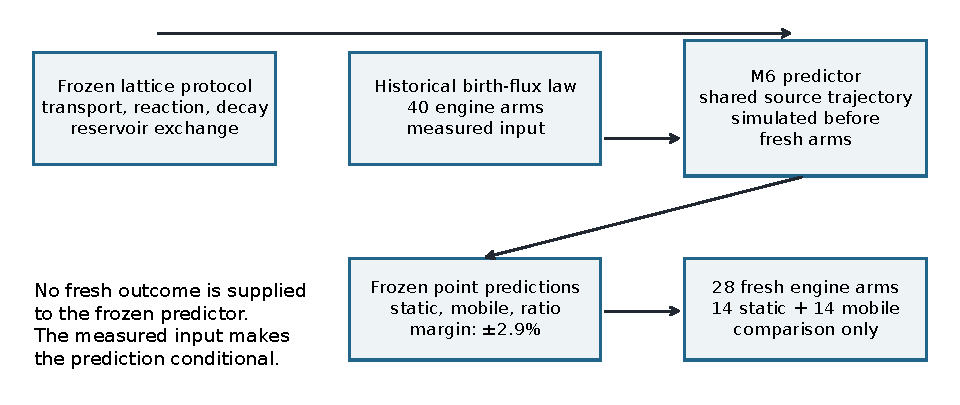
\includegraphics[width=\textwidth]{fig1_model_and_event_order.pdf}
\caption{Information supplied to the predictor and used for comparison. This is a schematic
of the archived calculation, not a particle snapshot. The measured historical birth-flux
law is the conditioning input. Fresh outcomes enter only the comparison.}
\label{fig:flow}
\end{figure}


\subsection{Pre-run decision and later diagnostics}
The frozen decision for each primary endpoint is
$|\widehat\theta/\theta_{\rm pred}-1|\le0.029$.
The margin uses named model-error terms and a sampling allowance based on historical
dispersion. Its construction therefore uses historical information.
The seed allocation, point predictions, tolerance and an ablation ranking rule were present
in Git before the fresh-arm commit. Fourteen load-bearing files match the freeze byte for byte.
This is a verified repository sequence, not a claim of independent public time-stamping.

The adjudication implementation and whole-interval rules appeared after the fresh runs.
Normal intervals, Student-$t$ diagnostics and equivalence-test probabilities must consequently
be labelled post-freeze. A point tolerance is not a pre-registered statistical equivalence
test \citep{wellek2010}. We retain the point decision as the criterion of record and report
sampling and predictor uncertainty separately. The supplement gives diagnostic arithmetic
without promoting it to a prospective endpoint.

\subsection{Audit and reconstruction}
We verified source hashes against pinned Git objects, recomputed arm summaries from all
28 raw NPZ files, checked frame counts and cadence, and reconstructed each final-state digest.
We independently recomputed the final radius from each final lattice.
The archives contain per-frame summaries and a final lattice, not every intermediate lattice;
the present audit does not independently reconstruct every frame radius from particle states.
No engine trajectory was rerun.

Historical inclusion sensitivity was recomputed from existing OBDI02 and OBTC02 archives.
Predictor-uncertainty and birth-flux comparisons use the stored SEAL01 arrays:
16 replicas of the 30-arm predictor calculation in each archived condition.
These are existing predictor calculations, not additional physical-engine confirmations.
All figures and tables are regenerated by the accompanying scripts.

\section{Results}
\subsection{The frozen predictions satisfy the point criterion}
All 28 declared fresh arms are present and included. None is recorded as extinct.
The raw arrays reproduce the archived medians, means, within-arm dispersions and blocking
fractions. Table~\ref{tab:primary} gives the primary comparison and the stored predictor
Monte Carlo dispersion. Figure~\ref{fig:fresh} displays each arm.

\begin{table}[htbp]\centering\small
\caption{Primary point comparisons. Monte Carlo s.d. is reported in percent as in SEAL01;
it describes repeated predictor calculations, not variation among engine arms.
The ratio dispersion uses the archived propagation convention.}\label{tab:primary}
\begin{tabular}{lrrrr}\toprule
Endpoint & Predicted & Observed & Error (\%) & MC s.d. (\%)\\\midrule
Static & \VStaticPredicted & \VStaticObserved & \VStaticError & \VStaticMCSD\\
Mobile & \VMobilePredicted & \VMobileObserved & \VMobileError & \VMobileMCSD\\
Mobile/static & \VRatioPredicted & \VRatioObserved & \VRatioError & \VRatioMCSD\\\bottomrule
\end{tabular}
\end{table}

The three point deviations are inside $\pm\VMargin\%$.
The sealed disposition is
\begin{quote}\small
\path{CONDITIONAL_FULL_CAPACITY_SOURCE_RESPONSE_OPERATOR_QUALIFIED}
\end{quote}
The label records this bounded result; it does not imply an exact theory of capacity effects.

\begin{figure}[htbp]\centering
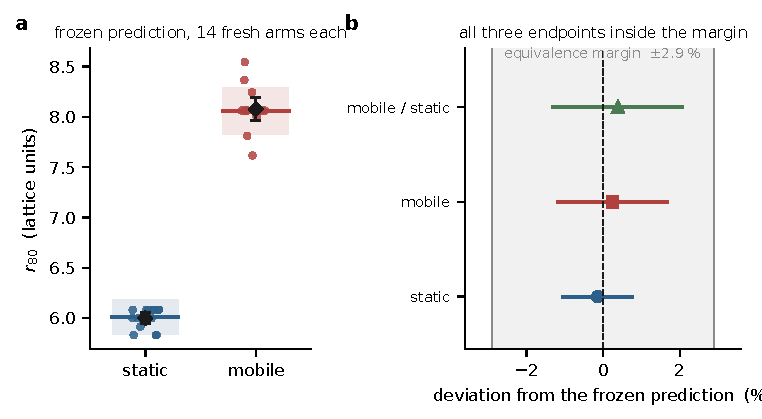
\includegraphics[width=\textwidth]{fig2_prospective_confirmation.pdf}
\caption{Fresh comparisons. (A) Each dot is one arm median; the horizontal red mark is the
frozen M6 prediction, and the black diamond is the observed condition mean with one standard
error across arms. (B) Point deviations for M6 and the historical-copy baseline. The band
shows the frozen tolerance, not a confidence interval. The baseline comparison is a later
diagnostic. Both predictors pass all three point criteria.}\label{fig:fresh}
\end{figure}


\subsection{Agreement does not uniquely identify the predictor}
A baseline that copies historical condition means gives fresh deviations of
\VBaselineStaticError\%, \VBaselineMobileError\% and \VBaselineRatioError\%.
All also satisfy the frozen tolerance. The baseline uses three static historical arms and
41 mobile historical arms at the same lattice size; it contains no transport model.
It was evaluated in the later seal. Its inputs existed before the fresh runs, but this
comparison was not itself a pre-run primary endpoint.

The fresh mobile observation differs by \VNoSharedError\% from the construction with the
shared source path removed, and by \VIdealError\% from the uncorrected ideal reference.
These fixed alternatives lie outside the point tolerance (Figure~\ref{fig:ablations}A).
The pre-run ablation rule required the full construction to be closer than the no-shared-path
variant; it did not prescribe a new statistical model-selection test.
Thus the comparisons support retaining a shared path within the examined construction,
while the successful historical baseline prevents a claim of unique mechanistic identification.

\subsection{The earlier birth-flux-shape interpretation is withdrawn}
The frozen Poisson-source variant is farther from the fresh mobile mean than M6, but it
still passes the same point tolerance. A ratio of distances is not evidence that it is rejected.
Stored SEAL01 replicas give mobile predictor residual means of \VEmpiricalMean\% for the
empirical flux and \VPoissonMean\% for the Poisson flux.
Their difference is $\VBirthDifference\pm\VBirthSE$ percentage points (one standard error;
Figure~\ref{fig:ablations}B). The earlier large effect had the opposite sign.
It cannot support the former causal attribution to birth-flux shape or the corresponding
factorial decomposition. A smaller effect is unresolved by the present account.
Conditionality remains, because the predictor still requires the measured input.

\begin{figure}[htbp]\centering
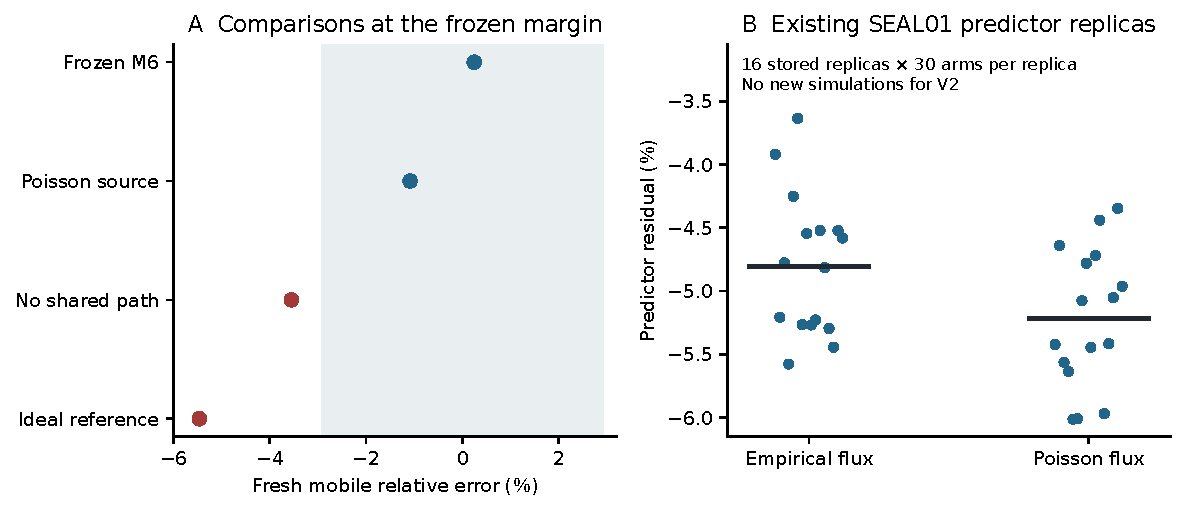
\includegraphics[width=\textwidth]{fig4_mechanism_ablation.pdf}
\caption{Model comparisons and the withdrawn flux attribution. (A) Point errors relative
to four frozen constructions; the Poisson variant is inside the same tolerance as M6.
(B) Existing replica means from SEAL01, with 30 predictor arms per replica.
Horizontal lines are means over the 16 stored replicas. These are post-outcome predictor
diagnostics and are not additional fresh engine arms.}\label{fig:ablations}
\end{figure}


\subsection{The historical residual depends on inclusion}
The original developmental summary selected arms with a surviving source, terminal $X$
population at least 40 and at least 50 finite analysis frames.
Since terminal population is an outcome, the selected residual cannot be reported as an
unconditional property of the dynamics. Table~\ref{tab:filter} and Figure~\ref{fig:filter}
reproduce the existing sensitivity analysis.

\begin{table}[htbp]\centering\small
\caption{Historical mobile inclusion sensitivity. All rows retain final $Y\ge1$;
the last still requires a finite radius. Rows overlap and are not independent studies.}\label{tab:filter}
\begin{tabular}{lrrr}\toprule
Rule & Arms & Residual (\%) & SE (\%)\\\midrule
Terminal $X\ge40$, at least 50 frames & \VSelectedN & \VSelectedResidual & \VSelectedSE\\
At least 50 frames & \VNoPopulationN & \VNoPopulationResidual & \VNoPopulationSE\\
At least one finite radius & \VFiniteOnlyN & \VFiniteOnlyResidual & \VFiniteOnlySE\\\bottomrule
\end{tabular}
\end{table}

The magnitude changes substantially as the filter is relaxed.
The widest row includes nearly extinguished fields and has larger uncertainty.
It does not prove a zero residual. The 28 fresh arms do not undergo this selection:
all declared arms remain in the primary analysis.

\begin{figure}[htbp]\centering
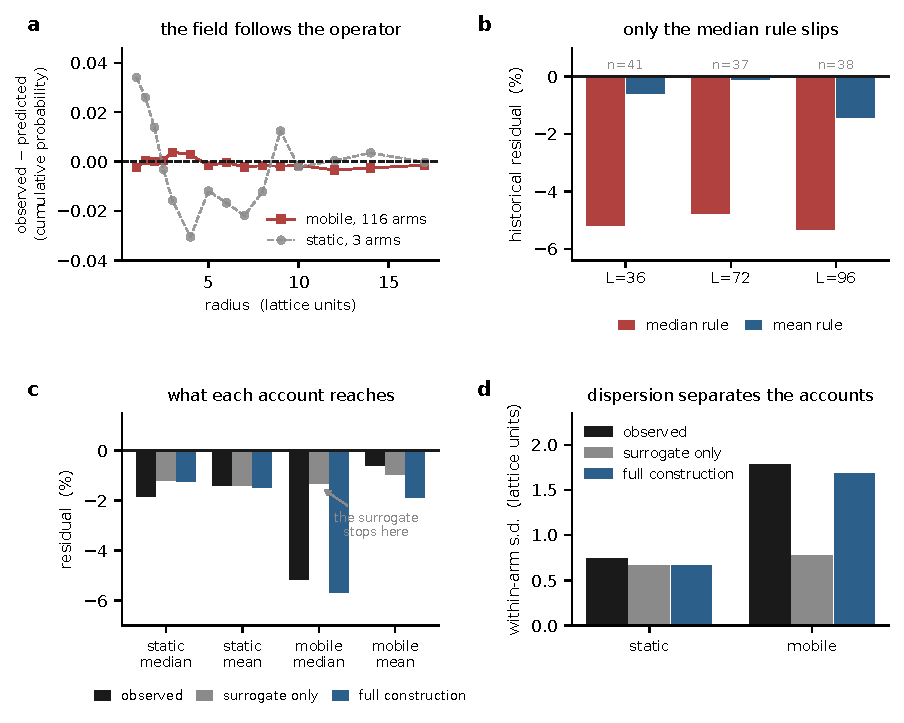
\includegraphics[width=.94\textwidth]{fig3_summary_rule_artefact.pdf}
\caption{Sensitivity of the historical radius summary to outcome-based inclusion.
Bars are one standard error across arms. Even the most permissive row is conditional
on an extant source and an available finite-radius summary.}\label{fig:filter}
\end{figure}


\section{Related results and limits of scope}
MYQBD01, PQEC01 and FLCR01 address the distinct problem of source succession and
two-centre organisation. MYQBD01 found organiser-only exposure insufficient to identify
the full descendant environment. PQEC01 retains \VPQArchives{} raw worlds, verified against
its manifest, but FLCR01 withdraws their prospective-confirmatory status because the
discovery/validation separation was not preserved. They are post-outcome developmental data.
FLCR01 rejects the necessity of a labelled founder's survival and supports a lineage
criterion, while retaining
\path{LINEAGE_CRITERION_SUPPORTED__OPERATOR_NOT_IDENTIFIED_FROM_PQEC01}.
A founder particle, a lineage, a source-response operator and a two-centre world are not
interchangeable units. None of these contextual findings extends the confirmation reported here.

EXP-SC-IOM-00 belongs to a separate scaffold-memory architecture. Its interpretive erratum
retains low-dimensional causal experience memory and explicitly records
\textbf{INDIVIDUATION: FAIL}. High-dimensional internal variation is not established
high-dimensional history storage. This result is included as a documentary boundary, using
its pinned report and erratum; its raw simulation was not rerun in this revision.
It is not evidence for individuality in the source-maintained lattice model.

The shared repository name does not make Route E, the persistence manuscripts or the
scaffold-memory architecture part of the present dataset. Their results are not pooled here.
Historical stop dispositions, including any
\path{STOP__ARCHITECTURE_CHANGE_REQUIRED}, remain attached to their originating experiments;
this paper neither reverses them nor exports them as a universal claim.
PMCR01 and the other closed routes are not reopened.

\section{Discussion}
The supported result is specific: a predictor conditional on a historical engine input
stated three point predictions before fresh engine outcomes existed, and
those outcomes satisfied its frozen tolerance. A fixed no-shared-path construction fails
the mobile point comparison, whereas both the full predictor and a historical-copy baseline
pass. The observation supports a useful construction at the tested settings but does not
uniquely identify the generating mechanism.

The audit changes two parts of the interpretation. First, a larger distance from an observation
does not imply model rejection when both distances satisfy the same rule.
Second, the historical residual combines the observable with an outcome-dependent inclusion
rule. A general theorem that a first-crossing quantile must be biased downward is not derived
here; the sign and magnitude of the observed summary effects remain empirical and conditional
on the analysed distributions.

Uncertainty also limits the apparent precision of agreement. The frozen numerical predictions
have Monte Carlo dispersion. Whole-interval rules and corrected small-sample diagnostics
were introduced after the runs and cannot be presented as pre-registered successes.
There is one engine implementation, one confirmatory lattice size, one parameter point and
two source-mobility conditions. No independent full-engine replication or general
parameter dependence is established.

For this paper, reproduction and heredity remain \textbf{NOT TESTED}; autonomous cohesion
and biological individuality remain \textbf{NOT ESTABLISHED}.
The external memory programme's individuation failure remains a failure.
This revision adds no experimental success and authorises no successor simulation.
Its contribution is a reproducible, narrower account of the source-response result and the
comparisons that limit what it can mean.

\section*{Data, code and provenance}
The review package includes the manuscript, supplement, claim--evidence matrix, deterministic
figure and table scripts, numerical reconciliation, source manifest and raw inputs needed
for its main figures. The source-response history is pinned at
\path{06c592313df96601de8d2a89676d5a5cf79fc414}; the original delivered paper is preserved in
Git at \path{0a872ac}. The V2 source and audit identify every included file by SHA-256.
PQEC01 raw archives remain a separately identified external package; their complete hash and
schema verification is supplied, while only their developmental status is used here.
The historical mission's governing run-budget authorisation is not in the delivered evidence;
its compliance remains \textbf{UNKNOWN}, which is not a finding of violation.
No publication, new DOI, public deposition or merge accompanies this revision.

\bibliographystyle{plainnat}
\bibliography{../bibliography/references}
\end{document}
